\documentclass[tikz,border=10pt]{standalone}
\usepackage{tikz}
\usetikzlibrary{positioning}

\tikzset{
  card/.style={draw=blue!70!black, line width=1.2pt, rounded corners=3pt, minimum width=3.5cm, minimum height=2.5cm, align=center, fill=none}
}

\begin{document}
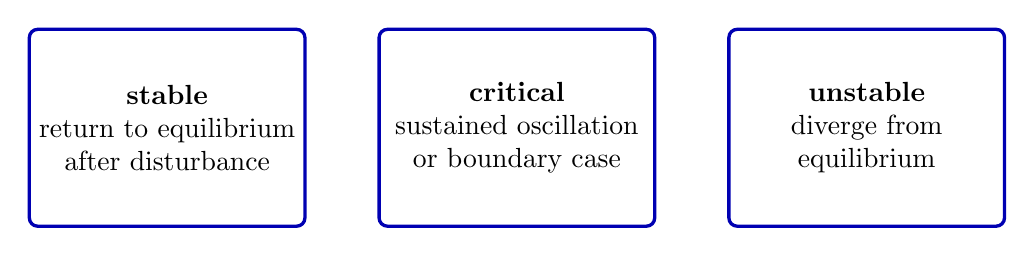
\begin{tikzpicture}[node distance=0.9cm]
  \node[card] (a) {\textbf{stable}\\return to equilibrium\\after disturbance};
  \node[card, right=of a] (b) {\textbf{critical}\\sustained oscillation\\or boundary case};
  \node[card, right=of b] (c) {\textbf{unstable}\\diverge from\\equilibrium};
\end{tikzpicture}
\end{document}
